\documentclass[a4paper]{article}

\usepackage{preambulo}
\usepackage{fancyhdr}
\pagestyle{fancy}
\usepackage{lastpage}

%\renewcommand{\chaptermark}[1]{\markboth{#1}{}}
\renewcommand{\sectionmark}[1]{\markright{#1}}

\fancyhf{}

\fancyhead[LO]{\rightmark}
\fancyhead[RO]{Trabajo Pr\'actico 2}
% \thesection\ 
\fancyfoot[LO]{\small{Sistemas Operativos}}
\fancyfoot[RO]{\thepage / \pageref{LastPage}}
\renewcommand{\headrulewidth}{0.5pt}
\renewcommand{\footrulewidth}{0.5pt}
\setlength{\hoffset}{-0.25in}
\setlength{\textwidth}{16cm}
%\setlength{\hoffset}{-1.1cm}
%\setlength{\textwidth}{16cm}
\setlength{\headsep}{0.5cm}
\setlength{\textheight}{25cm}
\setlength{\voffset}{-0.4in}
\setlength{\headwidth}{\textwidth}
\setlength{\headheight}{13.1pt}

\renewcommand{\baselinestretch}{1.1}  % line spacing

\begin{document}

\titulo{Trabajo Práctico 2}
\subtitulo{Algoritmos en sistemas distribuidos}
\materia{Sistemas Operativos}
\keywords{fqweeljk;lnrqefw}%TODO}

\integrante{Dandois, Santiago José}{105/17}{santids97@gmail.com}
\integrante{Tarzia, Chiara}{368/17}{dulcechiara@gmail.com}
\integrante{Zeitoune, Giselle Elizabeth}{121/17}{gisellezeitoune@gmail.com}

\abstract{freqwkl,;%TODO  En este trabajo práctico se busca modelar dos problemas distintos utilizando grafos como herramienta conceptual. El primer
problema, es el de la segmentación de imágenes, el cual resolvimos
utilizando un algoritmo similar al de generación de árbol mínimo.
El segundo problema, es un problema de optimización el cual se
resuelve buscando el camino mínimo en un grafo no trivial. En ambos
problemas, se
experimentó con distintas implementaciones e instancias para
comparar la performance de cada una de ellas. En el de segmentación
además se realizó un análisis cualitativo de las imágenes obtenidas.}

\maketitle

\tableofcontents
\newpage

\section{Introducción}

% Se introduce el problema, se muestra un review
% de la literatura y otros aspectos introductorios como posibles
% aplicaciones.


% \subsection{Se espera}
% Describir detalladamente el problema a resolver dando ejemplos
% del mismo y sus soluciones.


En este trabajo pr\'actico buscamos trabajar con sistemas distribuidos, sobre todo env\'io de mensajes utilizando la interfaz MPI.







\subsection{Blockchain}
El Blockchain consiste en un conjunto de bloques enlazados, en los que cada uno tiene:
\begin{itemize}
	\item \textit{\'Indice:} El n\'umero de bloque.
	\item \textit{Due\~no:} El identificador de qui\'en cre\'o el bloque.
	\item \textit{Dificultad:} La cantidad de ceros que debe tener el inicio del hash.
	\item \textit{}
	\item \textit{}
	\item \textit{}
	\item \textit{}
\end{itemize}

\subsection{Desarrollo}



Importante: Desarrolle un análisis del protocolo descrito en este trabajo que responda, al menos, a las siguientes preguntas:

¿Puede este protocolo producir dos o más blockchains que nunca converjan?

¿Cómo afecta la demora o la pérdida en la entrega de paquetes al protocolo?

¿Cómo afecta el aumento o la disminución de la dificultad del Proof-of-Work a los conflictos entre nodos y a la convergencia? Pruebe variando la constante DEFAULT_DIFFICULTY para adquirir una intuición.




\section{Experimentación}
En esta sección experimentaremos variando la dificultad del Proof-Of-Work y la cantidad de nodos, y mediremos el tiempo de ejecución. Para correr la experimentación se utilizó una computadora con un procesador \textit{Intel(R) Core(TM) i7-8550U CPU @ 1.80GHz} con cuatro cores.

\begin{figure}[H]
	\centering
	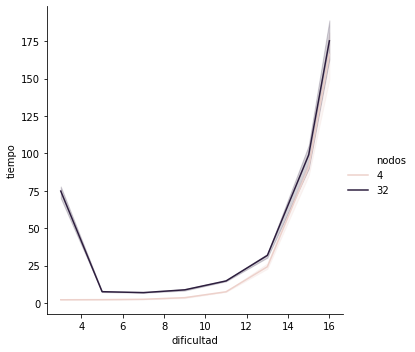
\includegraphics[width=0.7\linewidth]{img/grafico}
	\caption{Tiempo en función de dificultad para distinta cantidad de nodos.}
	\label{fig:grafico}
\end{figure}

En la Figura \ref{fig:grafico} podemos ver que cuando hay pocos nodos, el tiempo de ejecución crece muy rápidamente al subir la dificultad. En cambio, cuando hay muchos nodos, con dificultades muy chicas el tiempo es mayor y a medida que la dificultad aumenta, este disminuye hasta un punto en el que vuelve a aumentar.

Este comportamiento coincide con lo esperado a partir de nuestro análisis del protocolo. Cuando hay pocos nodos, 
la carga sobre la red es pequeña, sin importar la dificultad,
la cual varía que tan rápido se generan nuevos bloques. Luego el tiempo de generación de bloques se vuelve 
predominante sobre el tiempo de sincronización.

Cuando hay muchos nodos y la dificultad es baja,
es mayor el tiempo que se necesita para sincronizar las cadenas, a la vez que muchos bloques son 
desperdiciados. Al aumentar la dificultad, la cantidad de mensajes se reduce, y el tiempo necesario
para la sincronización también, luego el tiempo de producción de bloques se vuelve nuevamente predominante.
Es por esta razón, que vemos al tiempo de ejecuci\'on primero disminuir y luego volver a aumentar. A largo plazo, dado que la dificultad crece de forma exponencial, el tiempo de sincronizaci\'on se vuelve despreciable y es por esto que ambas curvas convergen.
\section{Discusión y conclusiones}

%Se discuten los resultados
%observados en la sección anterior y se da un cierre general.



\bibliography{biblio}

\end{document}
